\section{Resultados y Análisis}\label{sec:resultados2}

Se presentan los resultados de 30 corridas independientes de la Búsqueda Tabú con reinicio (Algoritmo~\ref{alg:tabu_ils}) sobre \textit{keller4} y \textit{C125.9}, con los parámetros especificados en la Sección~\ref{sec:met2}.

\subsection{Descripción de las instancias}

La Tabla~\ref{tab:instancias2} resume las instancias utilizadas. \textit{C125.9} se incorpora respecto al Informe 1 precisamente porque, siendo de menor tamaño que \textit{keller4}, es considerablemente más densa, lo que la vuelve más difícil para el método exacto (Sección~\ref{sec:contraste}) y permite evaluar la metaheurística en un régimen distinto.

\begin{table}[H]
\centering
\caption{Características de las instancias evaluadas.}
\label{tab:instancias2}
\begin{tabular}{lrrrr}
\hline
\textbf{Instancia} & \textbf{$|V|$} & \textbf{$|E|$} & \textbf{Densidad} & \textbf{$\omega(G)$ conocido} \\
\hline
keller4 & 171 & 9\,435 & 0.6491 & 11 \\
C125.9  & 125 & 6\,963 & 0.8985 & 34 \\
\hline
\end{tabular}
\end{table}

\subsection{Resultados agregados de las 30 corridas}

La Tabla~\ref{tab:resultados_meta} resume, para cada instancia, la tasa de éxito (fracción de corridas que alcanzó $\omega(G)$), el tamaño medio del clique encontrado, y el tiempo e iteraciones hasta alcanzar la mejor solución de cada corrida.

\begin{table}[H]
\centering
\caption{Resultados agregados de la Búsqueda Tabú con reinicio (30 corridas, semillas 0--29).}
\label{tab:resultados_meta}
\begin{tabular}{lrrrr}
\hline
\textbf{Métrica} & \textbf{keller4} & \textbf{C125.9} \\
\hline
Tasa de éxito ($f(S^*)=\omega(G)$) & 93.3\,\% (28/30) & 96.7\,\% (29/30) \\
Tamaño medio $\pm$ desv.\ estándar & $10.90 \pm 0.40$ & $33.97 \pm 0.18$ \\
Mejor tamaño observado & 11 & 34 \\
Tiempo medio hasta mejor solución & $0.0211 \pm 0.0458$ s & $0.0251 \pm 0.0385$ s \\
Iteraciones medias hasta mejor solución & 556.3 & 632.3 \\
\hline
\end{tabular}
\end{table}

En ambas instancias, la metaheurística alcanza el óptimo conocido en la gran mayoría de las corridas. En \textit{C125.9}, la única corrida que no lo alcanza se queda a un solo vértice de distancia ($f(S^*)=33$). En \textit{keller4}, de las dos corridas que no alcanzan el óptimo, una se queda a un vértice de distancia ($f(S^*)=10$) y la otra a dos vértices ($f(S^*)=9$). El tiempo hasta la mejor solución es del orden de centésimas de segundo en ambos casos, con una dispersión (desviación estándar) comparable a la media, lo que refleja que algunas corridas requieren varias perturbaciones antes de alcanzar el óptimo, mientras que otras lo hacen en la primera fase de expansión voraz.

\subsection{Efecto del mecanismo de reinicio (experimento de ablación)}

Para cuantificar el aporte del mecanismo de perturbación tipo ILS, se repitió el experimento desactivando el reinicio (\texttt{stall\_limit}$\to\infty$), es decir, ejecutando una Búsqueda Tabú pura sobre las mismas 30 semillas. La Tabla~\ref{tab:ablacion} muestra el resultado.

\begin{table}[H]
\centering
\scriptsize
\setlength{\tabcolsep}{3pt}
\caption{Experimento de ablación: Búsqueda Tabú pura (sin reinicio) vs.\ con reinicio tipo ILS.}
\label{tab:ablacion}
\begin{tabular}{@{}lrrrr@{}}
\hline
 & \multicolumn{2}{c}{\textbf{keller4}} & \multicolumn{2}{c}{\textbf{C125.9}} \\
\textbf{Variante} & \textbf{Tasa éxito} & \textbf{Tamaño medio} & \textbf{Tasa éxito} & \textbf{Tamaño medio} \\
\hline
Sin reinicio (Tabú puro) & 73.3\,\% & $10.57 \pm 0.76$ & 66.7\,\% & $33.40 \pm 1.11$ \\
Con reinicio (Tabú+ILS)  & 93.3\,\% & $10.90 \pm 0.40$ & 96.7\,\% & $33.97 \pm 0.18$ \\
\hline
\end{tabular}
\end{table}

El reinicio por perturbación mejora la tasa de éxito en 20 puntos porcentuales en \textit{keller4} y 30 puntos en \textit{C125.9}, y reduce la desviación estándar del tamaño final en un 48\,\% en \textit{keller4} y en un 84\,\% en \textit{C125.9}. El efecto es más pronunciado en \textit{C125.9}, consistente con lo señalado en la Sección~\ref{sec:met2}: al ser una instancia más densa, la vecindad \textsc{Swap} genera más plateaus donde el Tabú puro puede quedar atrapado sin un mecanismo de diversificación explícito.

\subsection{Curvas de convergencia}

Las Figuras~\ref{fig:conv_keller4} y~\ref{fig:conv_c1259} muestran la evolución del mejor $f(S)$ encontrado a lo largo de una corrida representativa (la que tardó más iteraciones en alcanzar su mejor solución, para ilustrar el mecanismo de reinicio con la trayectoria más larga y visible) para cada instancia. En ambos casos se observa un patrón característico de \emph{plateaus}: la construcción voraz inicial alcanza rápidamente un clique maximal subóptimo, seguido de largos períodos sin mejora donde la Búsqueda Tabú explora la vecindad \textsc{Swap}, hasta que una perturbación desplaza la búsqueda hacia una región desde la cual es posible seguir expandiendo.

\begin{figure}[H]
\centering
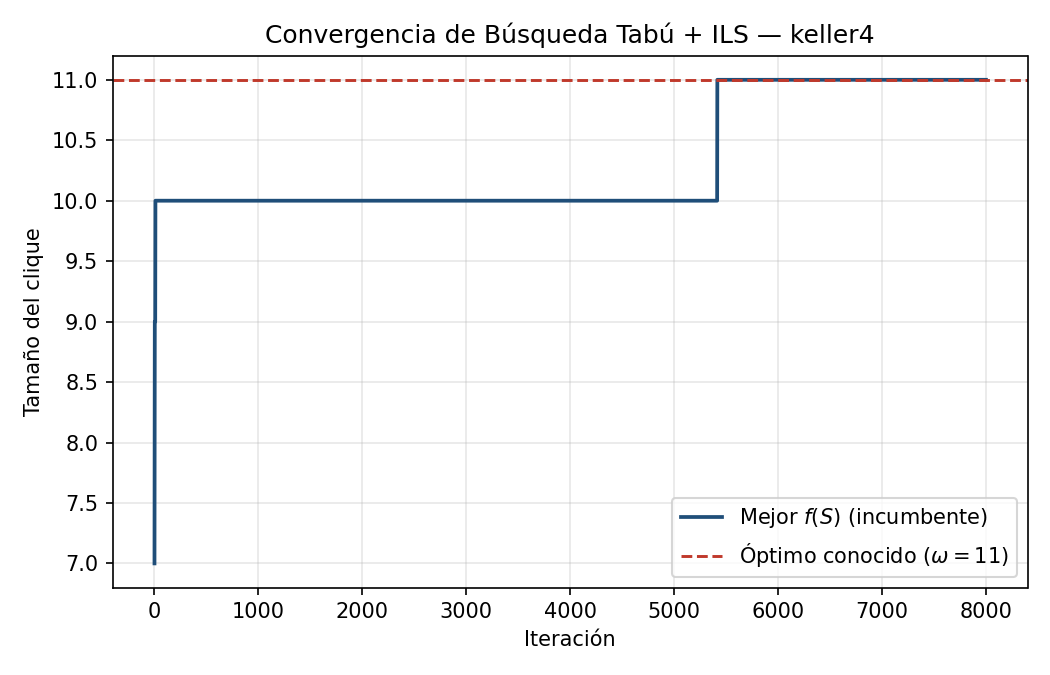
\includegraphics[width=0.8\textwidth]{../notebook_metaheuristica/convergencia_keller4.png}
\caption{Convergencia de la Búsqueda Tabú+ILS sobre \textit{keller4} (corrida representativa, semilla 20, 39 perturbaciones).}
\label{fig:conv_keller4}
\end{figure}

\begin{figure}[H]
\centering
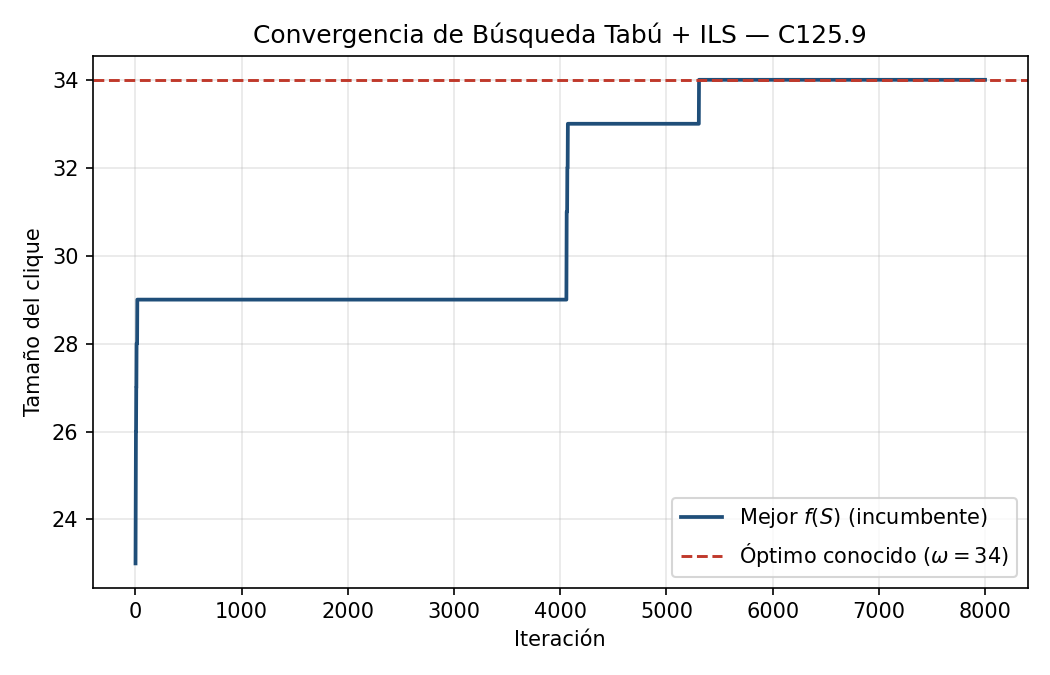
\includegraphics[width=0.8\textwidth]{../notebook_metaheuristica/convergencia_C125.9.png}
\caption{Convergencia de la Búsqueda Tabú+ILS sobre \textit{C125.9} (corrida representativa, semilla 8, 39 perturbaciones).}
\label{fig:conv_c1259}
\end{figure}

\FloatBarrier

\subsection{Visualización de las soluciones}

Las Figuras~\ref{fig:clique_keller4} y~\ref{fig:clique_c1259} muestran, para cada instancia, el grafo completo con el clique óptimo encontrado resaltado en rojo.

\begin{figure}[H]
\centering
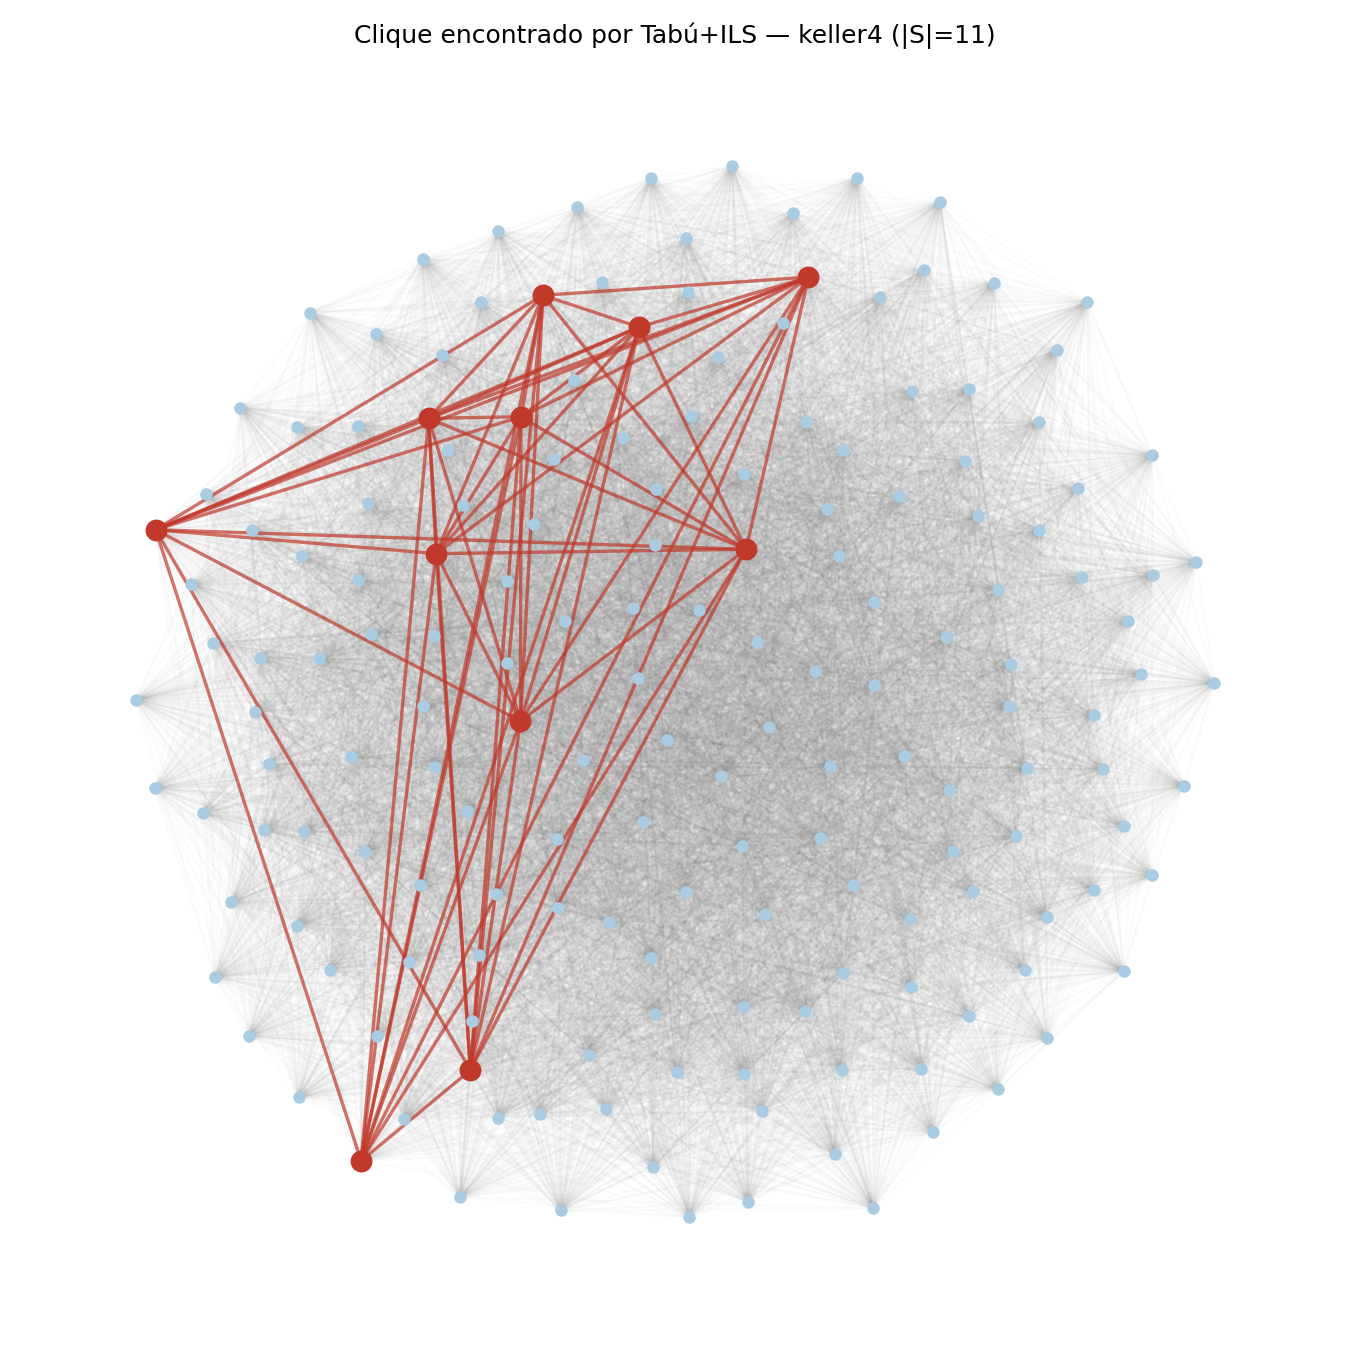
\includegraphics[width=0.62\textwidth]{../notebook_metaheuristica/grafo_clique_keller4_tabu.png}
\caption{Clique de tamaño 11 encontrado por Tabú+ILS en \textit{keller4}.}
\label{fig:clique_keller4}
\end{figure}

\begin{figure}[H]
\centering
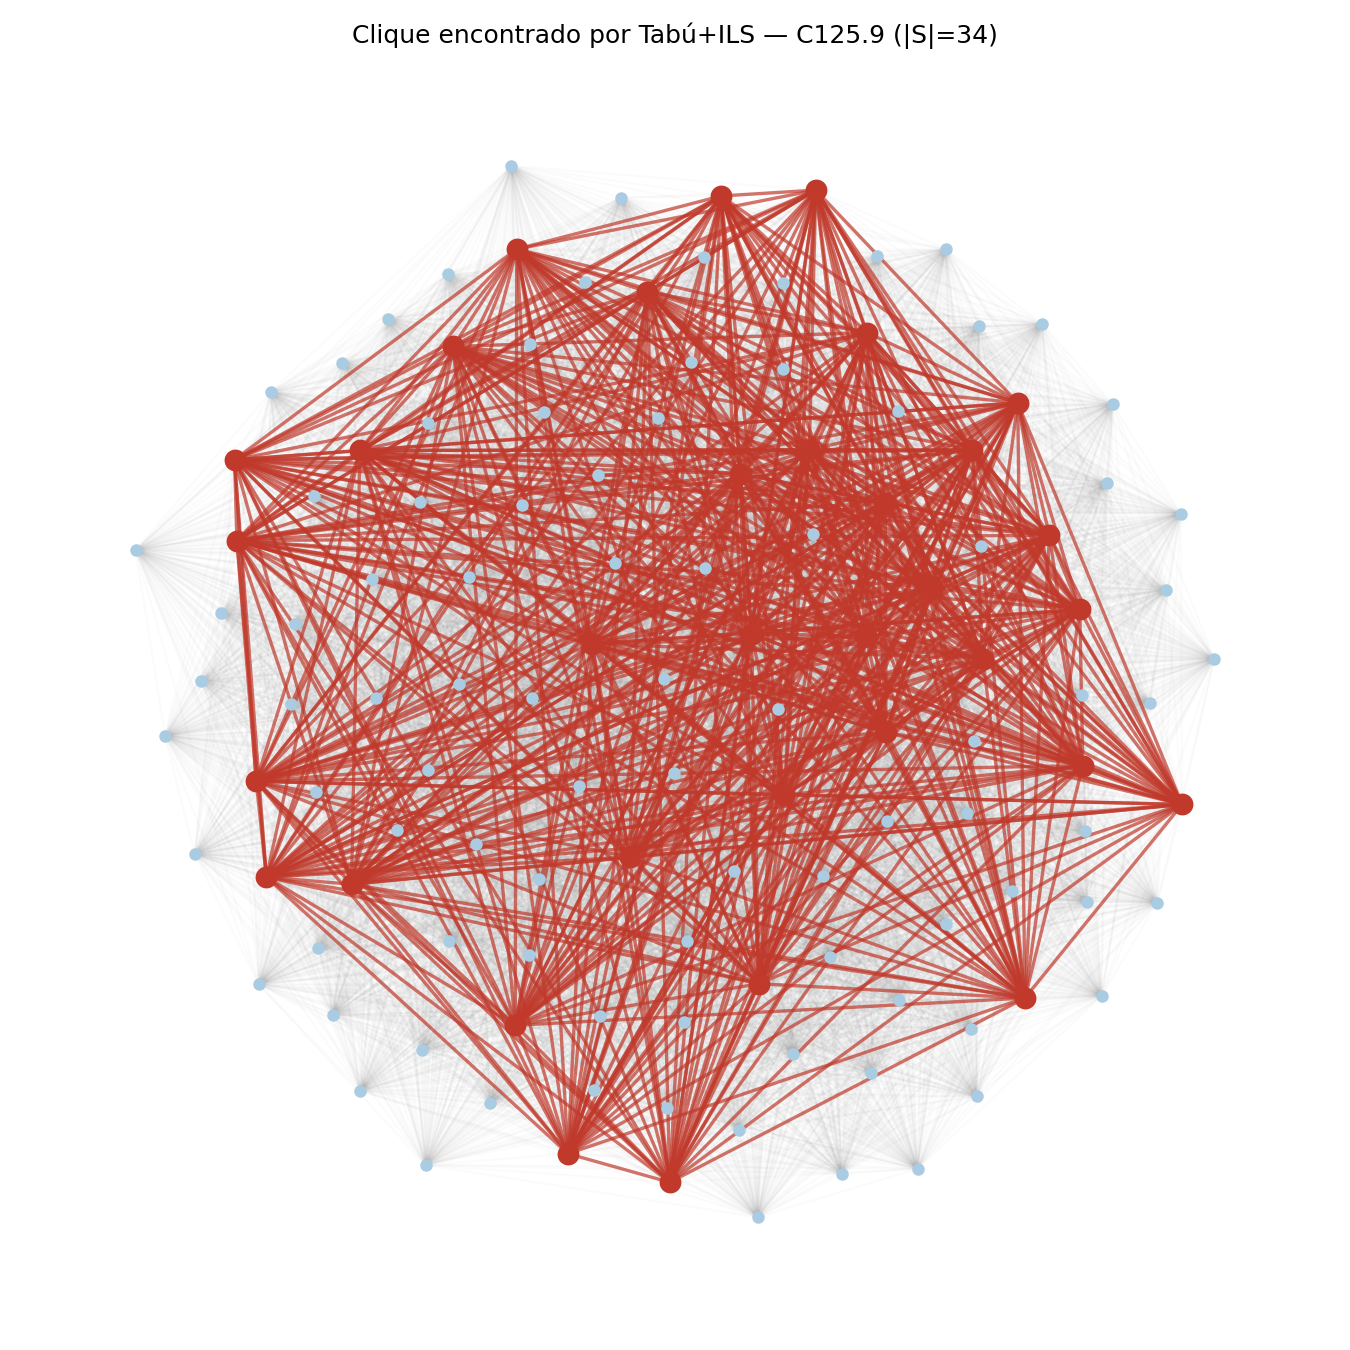
\includegraphics[width=0.62\textwidth]{../notebook_metaheuristica/grafo_clique_C125.9_tabu.png}
\caption{Clique de tamaño 34 encontrado por Tabú+ILS en \textit{C125.9}.}
\label{fig:clique_c1259}
\end{figure}
